\documentclass[tikz,border=20pt]{standalone}
\usetikzlibrary{calc}

\begin{document}
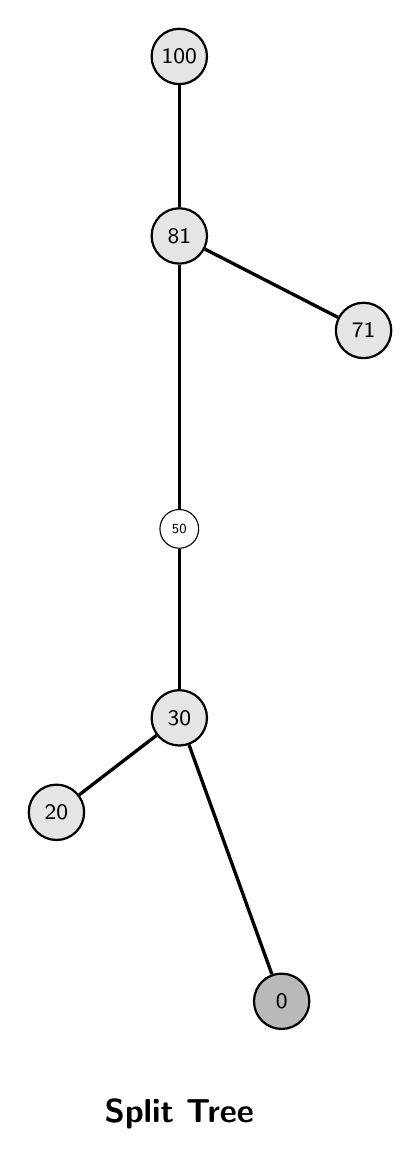
\begin{tikzpicture}[
    y=0.12cm, x=2.6cm,
    crit node/.style={circle, draw=black, fill=gray!20, thick, inner sep=1pt, minimum size=20pt, font=\sffamily\footnotesize},
    min node/.style={circle, draw=black, fill=gray!55, thick, inner sep=1pt, minimum size=20pt, font=\sffamily\footnotesize},
    reg node/.style={circle, draw=black, fill=white, inner sep=0.5pt, minimum size=14pt, font=\sffamily\tiny},
    main edge/.style={very thick, draw=black}
]

% Split Tree: 自下而上追踪子水平集 {f<=h} 的合并
% 关键点 = 极小值 (71,20,0) + split 鞍点 (81,30); 根 = 全局极大 (100)
% 退化为正则点: join 鞍点 50；非全局极大 90、80
\node[crit node] (P100) at (0.6, 100) {100};
\node[crit node] (P81)  at (0.6,  81) {81};
\node[crit node] (P71)  at (1.5,  71) {71};
\node[reg  node] (P50)  at (0.6,  50) {50};
\node[crit node] (P30)  at (0.6,  30) {30};
\node[crit node] (P20)  at (0.0,  20) {20};
\node[min  node] (P0)   at (1.1,   0) {0};

% 主干上行至全局极大 100 (途经正则点 50；局部极大 90/80 被剪枝)
\draw[main edge] (P30) -- (P50) -- (P81) -- (P100);

% split 鞍点 81: 极小值 71 的分量在此并入主干
\draw[main edge] (P71) -- (P81);

% split 鞍点 30: 极小值 20 与 0 在此合并
\draw[main edge] (P20) -- (P30);
\draw[main edge] (P0)  -- (P30);

\node[font=\sffamily\bfseries\large] at (0.6, -12) {Split Tree};

\end{tikzpicture}
\end{document}
